\documentclass[conference]{IEEEtran}

\usepackage{graphicx}
\usepackage{float}
\usepackage{amsmath}

\usepackage{amssymb} 
\usepackage{caption}
\usepackage{tikz}
\usepackage{xparse}
\usepackage{environ}
\usepackage{aliascnt}

\newaliascnt{eqfloat}{equation}
\newfloat{eqfloat}{h}{eqflts}
\floatname{eqfloat}{Equation}
\renewcommand\IEEEkeywordsname{Keywords}
\newcommand{\approximately}{{\raise.17ex\hbox{$\scriptstyle\mathtt{\sim}$}}}
\DeclareCaptionType{equ}[][]

\newcommand*{\ClipSep}{0.2cm}%

\title{\LARGE \bf
Developing a Robotics Quadruped Platform For Education}


\author{Keion Bisland$^{1}$ and Kai Zhang$^{2}$% <-this % stops a space
\thanks{*This work was not supported by any organization}% <-this % stops a space
\thanks{$^{1}$Keion Bisland is with the Department of Robotics Engineering,
        Worcester Polytechnic Institute, 100 Institute Rd., Worcester MA 01609, USA
        {\tt\small kbisland@wpi.edu}}%
\thanks{$^{2}$Kai Zhang is with the Department of Robotics Engineering,
        Worcester Polytechnic Institute, 100 Institute Rd., Worcester MA 01609, USA
        {\tt\small hzhang10@wpi.edu}}%
}


\begin{document}



\maketitle
\thispagestyle{empty}
%\pagestyle{empty} % this should be put back i jkust need page numbers to see length quickly
\pagestyle{plain}

%%%%%%%%%%%%%%%%%%%%%%%%%%%%%%%%%%%%%%%%%%%%%%%%%%%%%%%%%%%%%%%%%%%%%%%%%%%%%%%%
\begin{abstract}
	This paper introduces a novel way to teach kinematics, control, dynamics, trajectory planning, gait generation and many other core topics in robotics using the educational robotic platform developed, SmallKat. Like many other quadrupedal robotic platforms SmallKat uses 3 DOF legs allowing for motion in all 3 axes. The size, modulatiry, cost and capabilities of the robot are what suit it perfectly to teaching classes at a variety of levels. With the integrated sensing and safety features this platform is capable to satisfying classrooms from the undergraduate through he graduate level. The current educational environment has no means of educating the general school community effectively and affordably.
	\newline

\end{abstract}

\begin{IEEEkeywords}

    Quadruped, Low cost, Real time, Education, Dynamics, Controls, Micro Controller, Trajectory Generation, Inverse Kinematics, Forward Kinematics. DH-Parameters. 

\end{IEEEkeywords}

%%%%%%%%%%%%%%%%%%%%%%%%%%%%%%%%%%%%%%%%%%%%%%%%%%%%%%%%%%%%%%%%%%%%%%%%%%%%%%%%
\section{Introduction}
Looking into the available courses in Universities in the United States that offer courses and/or degrees in Robotics Engineering. This list encapsulated upwards of 100 Universities at the time of writing. Looking into the series of courses offered bu a number of the top universities on the list there is a distinct limit to the educational resources provided. Many of the schools cover courses in mobile robotics as there are a number of platforms available for purchase at a price feasible to use in a lab setting such as the Turtle bot 3 burger at a price point of \approximately\$550. This makes it affordable to provide lab groups with their own robot to work with, without the fear of damage to the platform. Robots with this same concept have been developed internal to many universities to teach a variety of topics, such as the 3-DOF robotic arm developed at WPI for its Unified Robotics III: manipulation course. Due to the development time and cost many universities tend to look for off the shelf solutions with supported materials and documentation to use in their classes. This in turn limits the variety of education received at different universities and relies of availability of platforms to expand the course curriculum. Due to this quadruped robotics have been limited to research labs (eg. \cite{8593885},\cite{HyQ}) with large restrictions on what can and cannot be done with the platform. Generally the platform for research is developed within the lab and costs far more than would be feasible to provide to lab groups. Even quadruped robots targeted at being low cost (eg. \cite{8793865},  \cite{Geva2014AND}) result in a platform costing many thousand dollars.  In order to overcome this the SmallKat platform was developed to meet a price point similar to the Turtle bot 3 and encapsulate concepts from all areas of robotics including Kinematics, Dynamics, Controls, Trajectory planning and Gait generation. The platforms sensing and modulatrity in turn extends itself to topics such as artificial intelligent, Human robot interactions and social robotics. 

\begin{figure}[t]
	\centering
      \begin{tikzpicture}
\node [inner sep=0pt] at (0,0) {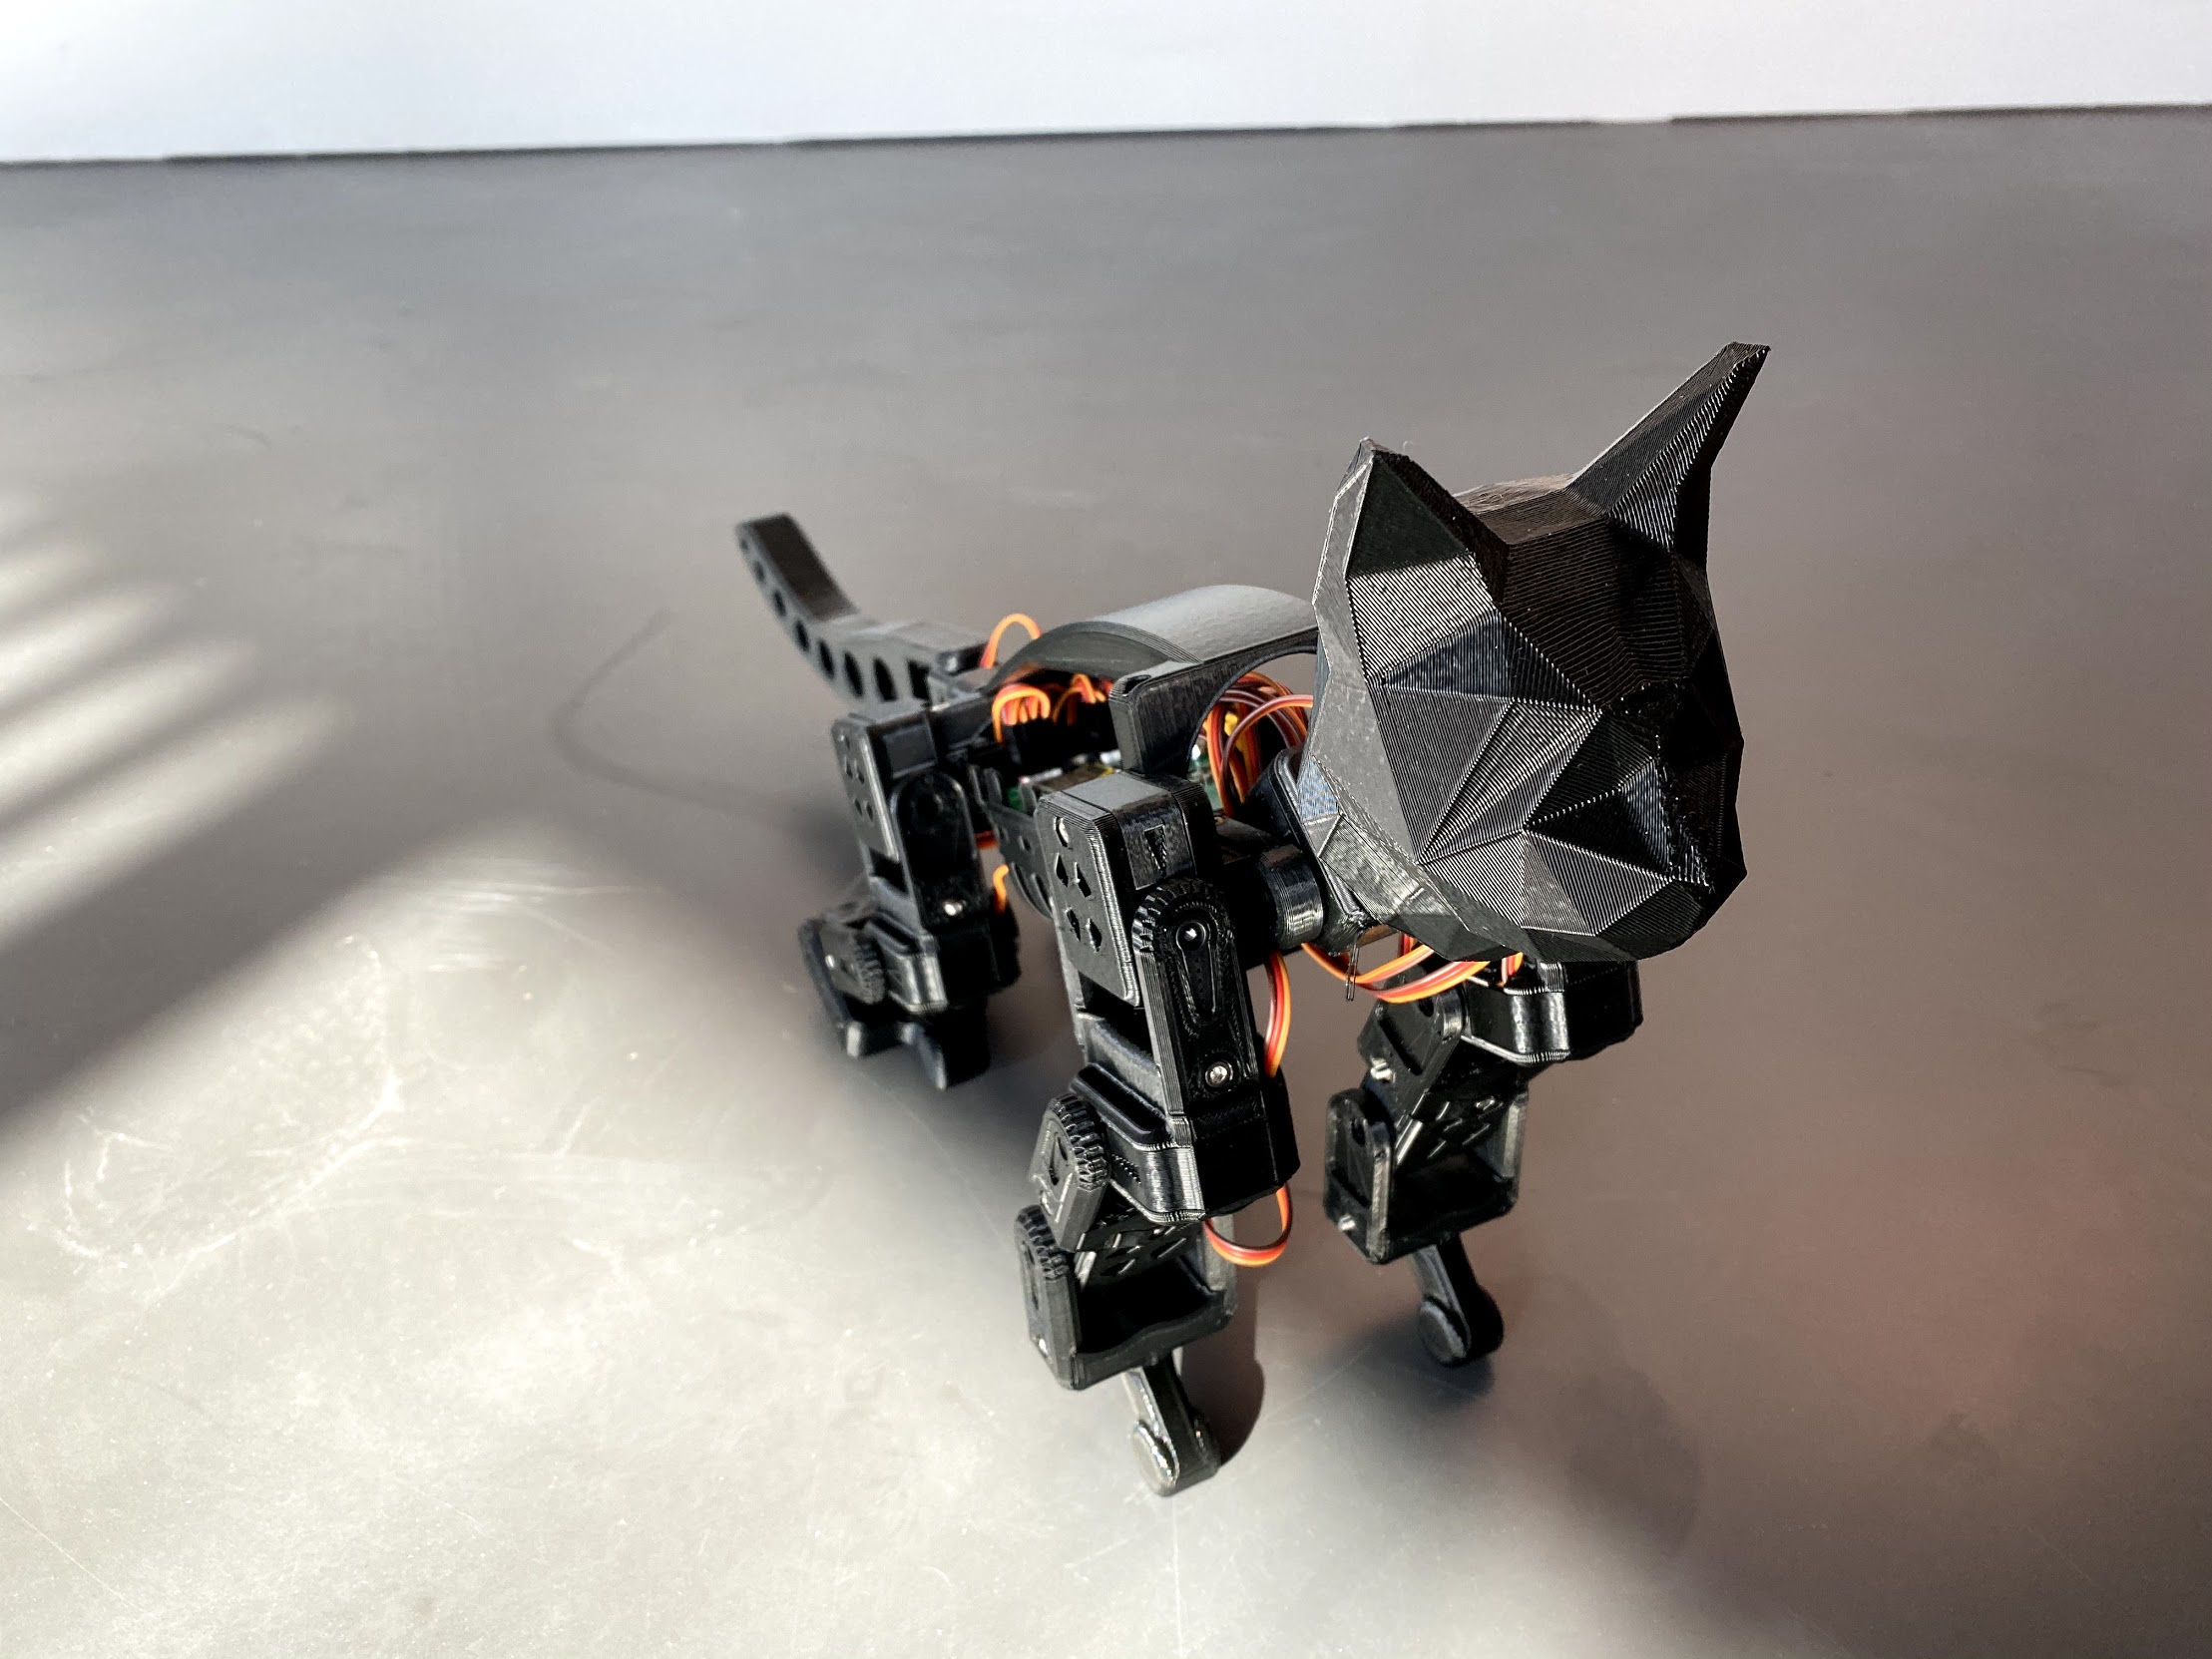
\includegraphics[width=0.4\textwidth]{Images/IMG_0119.jpg}};
\draw [white, rounded corners=\ClipSep, line width=\ClipSep] 
    (current bounding box.north west) -- 
    (current bounding box.north east) --
    (current bounding box.south east) --
    (current bounding box.south west) -- cycle
    ;
\end{tikzpicture}
  	\caption{Robot}
	\label{fig:FinalRobot}
\end{figure}
%%%%%%%%%%%%%%%%%%%%%%%%%%%%%%%%%%%%%%%%%%%%%%%%%%%%%%%%%%%%%%%%%%%%%%%%%%%%%%%%
\subsection{Related work and Background}
% I need to do the lit review on all of these
Despite the number of highly capable quadrupedal platforms existing in the education and research space such as \cite{8593885}, \cite{HyQ}, \cite{8793865}, \cite{8813480} and many more. Many of these platforms share a common theme of being very expensive, large and limited access with even the cheapest of the above listed costing in excess of \$3600 each \cite{8793865}. This makes the platforms highly capable, but completely infeasible to use in a classroom setting for undergraduate students. However from these publications a lot of controls knowledge, design details and requirements can be learned and advanced. Due to the size and weight targeted for the platform being developed a number of the control schemes designed mirror that of the cheetah mini robot\cite{8793865}. In that the limbs of both robots have so little inertial effect on the motion of the system that torque control of the limbs would not be highly effective. 

In development of an educational tools the work done by Naves Cocota et al.\cite{6900173} proved to be very useful in analyzing the requirements and solutions for the course material and testing. In combination with the work done to research the needs and effectiveness of educational robots \cite{8001854} provided a deep insight into the view of a number of groups on robot and their place in the educational work space. From this work it can be gathered that \approximately20\% of people surveyed by the group think that educational robots are very important to have at a variety of levels.

In the research space there are a number of small and some low cost quadruped research platforms such as \cite{Aracna}, \cite{shkolnik2010motion} and \cite{77248}, however many of these use a limited DOF configuration, either forcing them to use a design more resembling a spider \cite{Aracna} instead of a standard quadruped or are unable to perform dynamic motions and turns. This limits the pedagogical approach that can be taken using these platforms by limiting heavily what can be done. Others utilize 3 DOF legs, however they use very expensive closed loop servo motors, making it infeasible to produce a large number of them for a class.


Though there are a large number of universities offering courses in the robotics field, 10 universities were chosen for this study. The universities chosen have upstanding reputations in some and or all of the three major sub sections of robotics, Electrical Engineering, Computer Science and Mechanical Engineering or have an outstanding Robotics Engineering program, encapsulating all of these fields and more. The universities chosen include:


\begin{itemize}
     \item Worcester Polytechnic Institute\cite{wpiCourses}
    \item University of Pennsylvania\cite{uPennCourses}
    \item Oregon State University\cite{OreganStateCourses}
    \item Carnegie Mellon University\cite{CMUCourses}
    \item Johns Hopkins University\cite{JHUCourses}
    \item University of Michigan \cite{UMCourses}
    \item Cornell University\cite{CornellCourses}
\end{itemize}
\begin{figure}[H]
	\centering
      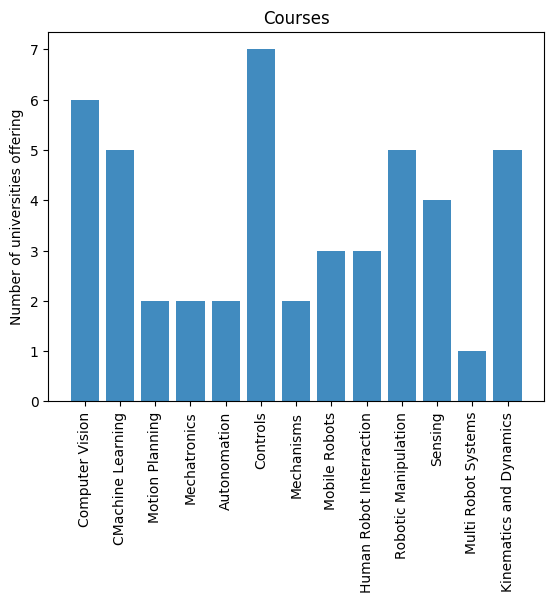
\includegraphics[width=0.4\textwidth]{Images/CourseOfferings.png}
  	\caption{Course content offered by number of universities}
\end{figure}

From this data, it can be seen most university's offer courses in mobile robotics, Controls, Kinematics and Robot Manipulation. Very few universities offer courses in multi pedal systems with none offering labs to undergraduate students. This limitation on course concepts is likely due to the lack of available hardware and course concepts on the market. 

%%%%%%%%%%%%%%%%%%%%%%%%%%%%%%%%%%%%%%%%%%%%%%%%%%%%%%%%%%%%%%%%%%%%%%%%%%%%%%%%
\subsection{Problem Statement}
Though there are upwards of 100 universities in the United States of America that offer courses and/or degrees in Robotics, there is a common missing course required for modern robotic systems. As technologies develop further more development will be done into quadruped and humanoid robots. Due to the lack of affordable, capable hardware it is increasingly hard to develop a course without hardware. In order to develop the hardware it requires an education on the material involved with it and to develop the course material it required hardware to develop with. In order to have engineers ready and capable development and work with multi-pedal robots a low cost and capable platform must be developed. 
In order to make this platform available t as many people as possible the overall price was kept as low as possible while not sacrificing on functionality. A small yet highly capable platform integrating a series of sensors was developed at a price point of \approximately\$250 in parts and manufacturing costs. This brings the price of a functional quadruped platform into the price point of many hobbyists and undergraduate lab budgets. This system integrates all necessary sensors and safety components to ensure longevity of the system and prevent harm and injury to the users. This paper will go through the design and manufacturing decisions of the entire system including the physical robot, simulation environment, electronics and sensors and the  code base to operate the entire system.


%%%%%%%%%%%%%%%%%%%%%%%%%%%%%%%%%%%%%%%%%%%%%%%%%%%%%%%%%%%%%%%%%%%%%%%%%%%%%%%%
\section{Design Requirements}\label{sec:DesignReqs}
In order to design the platform appropriately the teaching objectives had to be defined and considered in the development process. The sections proceeding cover all the topics covered and their relationship to the platform.
\subsection{Kinematics}
    In learning control and manipulation of a multi DOF system, Kinematics and Denavit–Hartenberg parameters are crucial. Through this series of equations and parameters all following concepts can be taught and tested sufficiently. A strong understanding of these concepts is crucial for any multi DOF and/or multipedal system.
    \paragraph{D-H Parameters}\label{DH-Params}
    D-H Parameters explain the configuration of each joint of the robot and its translation from the previous join tin a series of 4 Parameters. Through these parameters the forward kinematics of the system can be quickly and easily computed with very little modification in the case of a change to the system. Table \ref{tab:DHParametersLeg} shows the DH Parameters of the legs of the robot.
    
    \paragraph{Forward Kinematics}
    Forward Kinematics allow the robot to know the position in the X,Y,Z work space given the current joint angles. this can be approached in 2 ways. The geometric approach using a series of 3 equations seen in Equations \ref{FK:X}, \ref{FK:Y}, \ref{FK:Z} or using the D-H parameters in section \ref{DH-Params} and a homogeneous transformation matrix shown in figure \ref{mat:FKTransform}
    
    \paragraph{Inverse Kinematics}
    Inverse kinematics allow the controller to calculate the joint angles required to reach a certain target goal in the work space. These joint angles can be derived from a series on equations seen in equations \ref{IK:q1}, \ref{IK:q2} and \ref{IK:q3}.
   

In order to cover topics so important to the material for the course it was imperative that the kinematics for the system could be developed and tested on a single leg before testing on the whole robot. This was achieved through software integration allowing for individual joint control from the high level interface. This allows the users to develop their kinematic equations and test them in a simple and reliable way in order to get a solid understanding of the concept.

\subsubsection{Trajectory Generation}
 Following kinematics and preempting gait generation the topics involved in trajectory planning are of high importance. Understanding frame transformations and $n^{th}$ degree polynomials for path and trajectory generation will make the process of gait generation and motion planning far easier and more efficient. 

\subsubsection{Gait Generation}
 Following Trajectory generation comes gait generation. This covers the trajectories that must be followed for each leg in a specific sequence in order to achieve a specific body trajectory, moving the entire robot in a specific direction.

\subsubsection{Controls \& Dynamics}
  When developing a complex system controls and dynamics are crucial to have the robot accurately and safely perform tasks and actions commanded to it. The platform must be able to have both control systems and dynamic controllers implemented to account for external input from the environment.

%%%%%%%%%%%%%%%%%%%%%%%%%%%%%%%%%%%%%%%%%%%%%%%%%%%%%%%%%%%%%%%%%%%%%%%%%%%%%%%%
\section{Methodology and Implementation}

When developing the platform, a number of considerations were taken into account. Many of them were targeted in order to optimize for mass production and reliability. A platform given used for education must have a high degree of reliability and repair-ability. In order to make it feasible for a class setting the over all cost and part replacement costs must remain as low as possible without affecting the reliability of the system. Along with this a careful focus was placed on developing the supporting information for the platform including the teaching objectives   

In  order to ensure functionality the DH Parameters of the legs were optimized to allow for the longest leg length and there fore the longest stride length while still allowing for the motors to support the required force. In order to do this the torque jacobian for each of the legs was computed and  values were tested iteratively to achieve a torque of less than 3Kg/cm in the greatest case. This resulted in the DH parameter in table \ref{tab:DHParametersLeg} where link 0 is the translation from the center of the body to the first joint for each leg. 
\begin{table}[H]
    \centering
    \begin{tabular}{|c|c|c|c|c|}
    \hline
    Link& A  & $\alpha$ & D & $\theta$ \\
    \hline     
        0 &  0 & 0 & $\pm$151.42 &0\\
        1 &  0 & $-\pi/2$ & 45.5  &$\theta_1$\\
        2 &  0 & 0& 55.50 & $\theta_2-\pi/4$\\
        3 & 0  &0 & 60  &$\theta_3+\pi/2$\\
    \hline
    \end{tabular}
        \caption{\label{tab:DHParametersLeg}D-H Parameters of a single leg}
    \end{table}
    Following the DH Parameters the Forward and Inverse kinematic equations were calculated to begin simulation of the system. This resulted int he forward kinematics in Equation \ref{eq:FK} for the forward kinematics of each leg.
\begin{eqfloat}[H]
    \begin{equation}
        X = 
        \label{FK:X}
    \end{equation}
    \begin{equation}
        Y = 
        \label{FK:Y}
    \end{equation}
    \begin{equation}
        Z = 
        \label{FK:Z}
    \end{equation}
    \setcounter{equation}{0}
    \caption{\label{eq:FK}Forward Kinematics Equations}
    \end{eqfloat}
    These equations were then reduced to using the Homogeneous Transform matrix method in which the forward kinematics can be very quickly calculated using the DH Parameter Table \ref{tab:DHParametersLeg} and the Homogeneous Transform \ref{eq:HomogeneousTransform}
    \begin{eqfloat}[H]
        \centering
        $$
        \begin{matrix}
        C\theta_i & -S\theta_i & s\theta_iS\alpha_i &a_iC\theta_i\\
        S\theta_i& c\theta_i & -C\theta_iS\alpha_i & a_iS\theta_i\\
        0 & S\alpha_i & C\alpha_i & D_i\\
        0 & 0 & 0 & 1\\
        \end{matrix}
        $$
    \caption{\label{eq:HomogeneousTransform}Homogeneous Transformation}
    \end{eqfloat}
    From this the Inverse Kinematics were calculated to continue the simulation process. This resulted in the equations seen in Equation \ref{eq:IK} 
    
    \begin{eqfloat}[H]
    \setcounter{equation}{0}

    \begin{equation}
        \theta_0 = 
        \label{IK:q1}
    \end{equation}
    \begin{equation}
        \theta_1 = 
        \label{IK:q2}
    \end{equation}
    \begin{equation}
        \theta_2 = 
        \label{IK:q3}
    \end{equation}
    \setcounter{equation}{2}
    \caption{\label{eq:IK}Inverse Kinematics Equations}
    \end{eqfloat}
    
    These equations were then computed integrated with the trajectory generation and gait generator code developed and tested on the simulation robot using an environment called BowlerStudio\cite{BowlerStudio} using the bullet physics engine \cite{Coumans:2015:BPS:2776880.2792704}. A packet manager interfacing through UDP was implemented to communicate from the high level controller run in java on the main computer computing the gait, trajectories and kinematics for the system and reporting joint angles to the robot wirelessly. The robot then responds with the current system dynamics including the IMU data providing the Euler angles of the robot and the gravity vector showing exactly where how the robot is positioned and the current for each joint and any safety alert information coming from the safety processor including battery voltage and charge status. This control structure can be seen in \ref{fig:controStructure}.
    
    This separation onto two independent systems of High level code that can be tested in the integrated simulation environment and low level robot code allows for development and testing without having the physical robot and also allows for topics such as kinematics to be tested and validated before implementing on the physical robot which should lessen the chances of robot or user harm. This also allows for the exact same code to be run for both the simulation and physical robot with no change to the code.
    
    \begin{figure}[H]
	\centering
      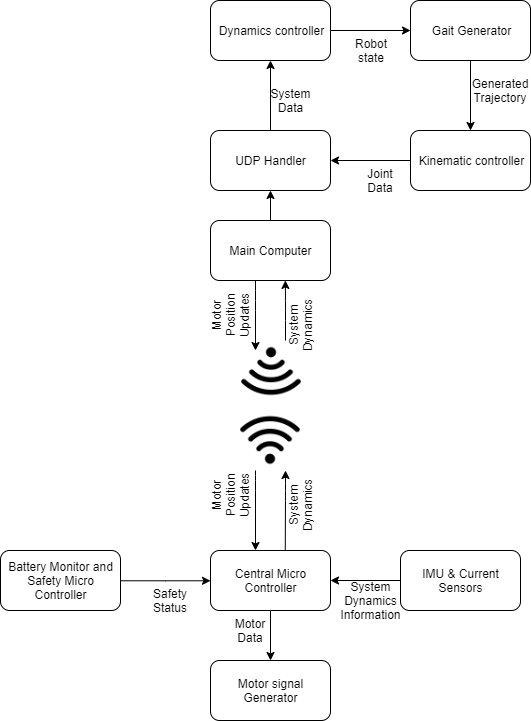
\includegraphics[width=0.4\textwidth]{Images/SmallKatControllerDiagram.png}
  	\caption{System Control Diagram}
  	\label{fig:controStructure}
\end{figure}

The resulting design can be see with all of the components, motors and electronics in the exploded view seen in figure \ref{fig:explodedView}. this view shows how the robot is constructed, all of the sub components and how that are used in different locations. The components selected and their choice reasons are consolidated in table \ref{tab:DesignDecisions}. For further information into these decisions Section \ref{sec:discussion}.


\begin{figure}[H]
	\centering
      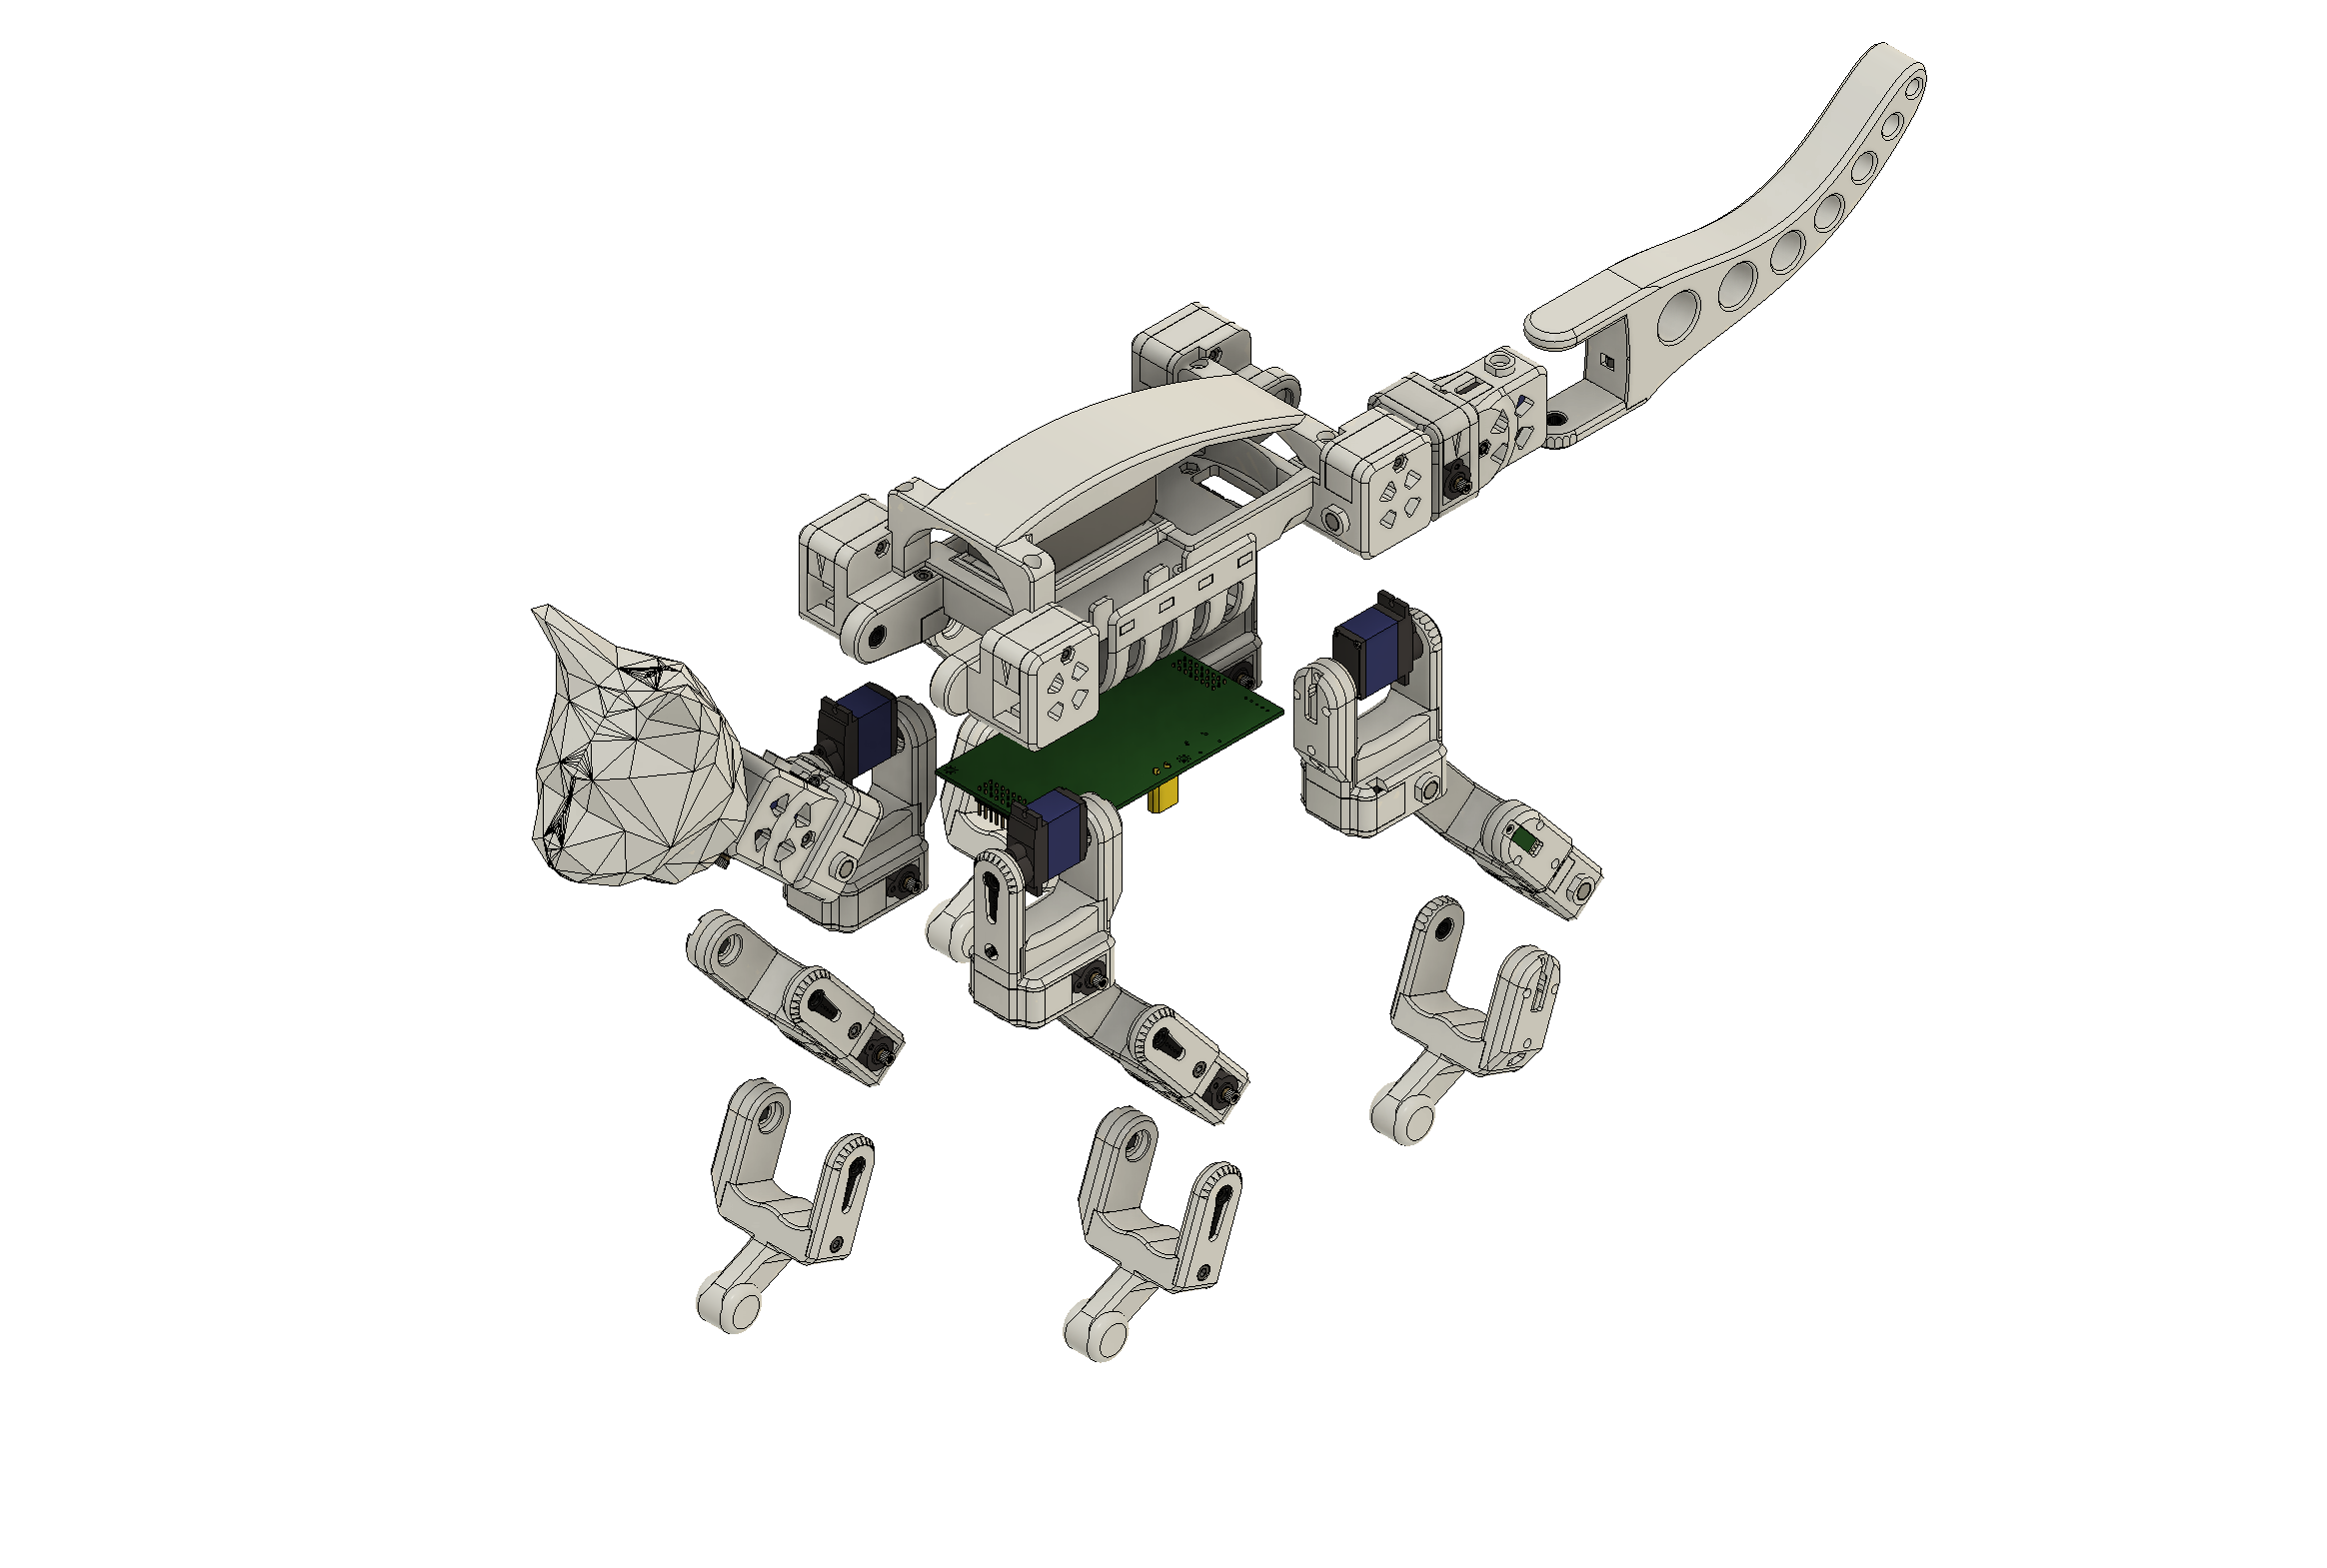
\includegraphics[width=0.5\textwidth]{Images/ExplodedView.PNG}
  	\caption{System Control Diagram}
  	\label{fig:explodedView}
\end{figure}

\begin{table}[H]
    \centering
    \begin{tabular}{|c|c|c|}
        \hline

    Component &  Choice & Reason for Choice \\
    \hline
    Motor & MG92B   &   \begin{tabular}{c}
                                         Low Cost\\
                                         Easily Available\\
                                         High Torque for form factor\\
                                    \end{tabular}\\
       \hline
     Micro Controller & ESP32   &   \begin{tabular}{c}
                                         Low Cost\\
                                         Easy Development\\
                                         Wireless capabilities\\
                                    \end{tabular}\\
       \hline   
    Safety Controller & STML432Kx   &   \begin{tabular}{c}
                                         Ultra low power\\
                                         High Reliability\\
                                         Small Form Factor\\
                                    \end{tabular}\\
     \hline   
    IMU & BNO055   &   \begin{tabular}{c}
                        Well Supported\\
                        Filtered Output\\
                        High Accuracy\\
                       \end{tabular}\\
       \hline   
    \end{tabular}
    \caption{Caption}
    \label{tab:DesignDecisions}
\end{table}


%%%%%%%%%%%%%%%%%%%%%%%%%%%%%%%%%%%%%%%%%%%%%%%%%%%%%%%%%%%%%%%%%%%%%%%%%%%%%%%%
% \section{Experiment}
% In order to prove the validity of the project a pilot study was conducted with 3 students at Worcester Polytechnic Institute where they would assemble, test and develop a stable walking gait using the platform and provided architecture. In order to collect data from the students through out the 7 week study, the students were asked to fill out an anonymous survey after every weeks material. The students within the study were provided with study and research materials and sample / starter code for each weeks lab session. They would then take this code and develop the weeks goal from there. Within the study the topic of kinematics, dynamics, trajectory planning and gait generation are covered in detail.  

%%%%%%%%%%%%%%%%%%%%%%%%%%%%%%%%%%%%%%%%%%%%%%%%%%%%%%%%%%%%%%%%%%%%%%%%%%%%%%%%
\section{Discussion}
\label{sec:discussion}
\subsection{Design}
\subsubsection*{Design Considerations}
\paragraph*{Mechanical}
    When designing the mechanical system for the robot, there were large number of constraints and hurdles to overcome. Many of the constraints can be refined down to the cost and the size constraints set forth during the development of the platform. 
    \begin{itemize}
        \item Motor selection- 
            When deciding motors to use there were a number of criteria to compare. 
            \begin{itemize}
                \item Size
                \item Torque
                \item Power requirements
                \item Availability
            \end{itemize}
            In end the 13g servo form factor was chosen for the size as it would allow the overall robot size to remain small and light as can be seen in [\ref{appendix:MotorSelection}]. It then came to choosing the specific motor to use, it came down to 4 motors. All of the considered motors were high torque variants using metal gears. due to sharing the same form factor they all remained in a very similar volumetric size so it came down to which motor would be most capable and reliable. After testing with all of the considered motors, the final motor chosen was the MG90B for its high size to torque ration, being far higher than the other options.\newline
        
        \item Manufacture-ability
        While designing this robot a great deal of time was spent in designing for manufacture-ability. Each method of manufacturing has different constraints in what can be produced successfully, efficiently and quickly. When designing a number of factors were considered. \newline
            \begin{itemize}
                \item Manufacturing style
                \item Number of components
                \item Production cost
            \end{itemize}
        The primary means of manufacturing was chosen as 3D printing because it would allow the robot to be iterated quickly and available to the most people. However for mass production of the platform, a series of molds would be created and parts would be cast using a poly-urethane resin. This required all parts to be designed with both in mind ensuring there were as few areas with unreachable overhangs, parts could be placed flat in order to reduce the amount of support material while printing and many other details. By choosing these two methods of manufacturing the overall production costs are kept very low.\newline
        Due to the nature of the system, there will be a high number of individual components (79 total parts in the final design), by reusing the same piece in multiple it both reduces the complexity of assembly and the total number of models that have to be manufactured. Through this technique, the robot was able to be designed out of 22 individually unique components which would be able to be printed in 3 cycles of a standard 200mm x 2000mm 3d printer (industry standard for non industrial printers).\newline
        \item Assemble-ability
        While manufacture-ability encapsulates the majority of the design process, the means of assembling was also considered carefully. The ability to put the robot together quickly and easily is critical. By analyzing the process taken to assemble an early prototype of the robot and adjusting the design the assembly time was reduced from \approximately 5hrs to \approximately1.5hrs. The final revision of the design utilized 2 lengths of m3 bolts and their corresponding nuts to assemble the whole robot. The use of 2 lengths of screws also drastically reduces the cost. 
        
    \end{itemize}
\paragraph*{Electrical}
The electrical system came down to a few major requirements. The robot requires many independent sub components with their supporting hardware

    \begin{itemize}
        \item Micro controller -
            When choosing the micro controller there were a few requirements set forth, it would have to be able to run 16 independent PWM channels through hardware, communicate through either USB-HID or UDP and have a dedicated hardware $i^2c$ bus. With these requirements a list of possible micro controllers was developed, ranging from off the shelf boards to completely custom hardware.
            \begin{enumerate}
                \item Teensy 3.5/3.6
                \item Teensy 4.0
                \item ESP32
                \item STM32
            \end{enumerate}
            From this list a custom motherboard was developed. From this list of micro controllers it was narrowed down to two choices being the Teensy 3.5 and the ESP32, one option providing hardware USB-HID and the other UDP. From this a final version of the motherboard was developed using the available boards. Both boards were then put into robots for testing. The ESP32 communicating directly with the high level controller over WiFi, the Teensy communicating with a Raspberry pi onboard the robot, running the high level controller. However due to a bug in the current Raspberry pi kernel and the USB HID library implemented in have the testing on the Teensy had to stop as it could not be tested in the assembled system in the intended way. This switch also reduced the overall price of the system by removing the cost of a dedicated Raspberry Pi and by using a much lower cost micro controller.\newline
            
        \item IMU- 
            The IMU chosen was the BNO055 as it contains an embedded M0 arm micro controller that filters the data coming out of the IMU. This allows the system to have a much more reliable source of data. The internal micro controller is also able to provide a gravity vector and the Euler angles within each axis of rotation.\newline
            
        \item Power regulation-
        Due to the power requirement of the motors chosen, a consistent 6v power supply with about 20A continuous current draw is required. 6v is a very uncommon voltage supply with 2s lithium batteries coming in at a nominal 7.4V and most bench power supplied only supplying up to 10A. In order to increase the battery life capacity without increasing the size of the cells as well as allowing for higher voltage power supplies with lower current ratings to be used a high current switch mode supply was designed with up to an 18V input and up to 20A output. With an overall efficiency of about 85\% at the full 20A draw the onbaord supply is highly efficient at converting high voltage, low current supplies down to 6v at the required 20A. \newline
    \end{itemize}
    During the development stages of the motherboard, off the shelf development boards and modules were used for the micro controller, IMU and power regulation. This drastically increased the overall cost of the electronics in the system. Once the system was proven and tested, the final revision of the motherboard was designed and resulted in a cost reduction of about 80\%. In addition to the cost reduction, The overall number of through hole components was drastically reduced, making it marginally easier to produce.
    
    
% \begin{figure}[H]
% 	\centering
%       \begin{tikzpicture}
% \node [inner sep=0pt] at (0,0) {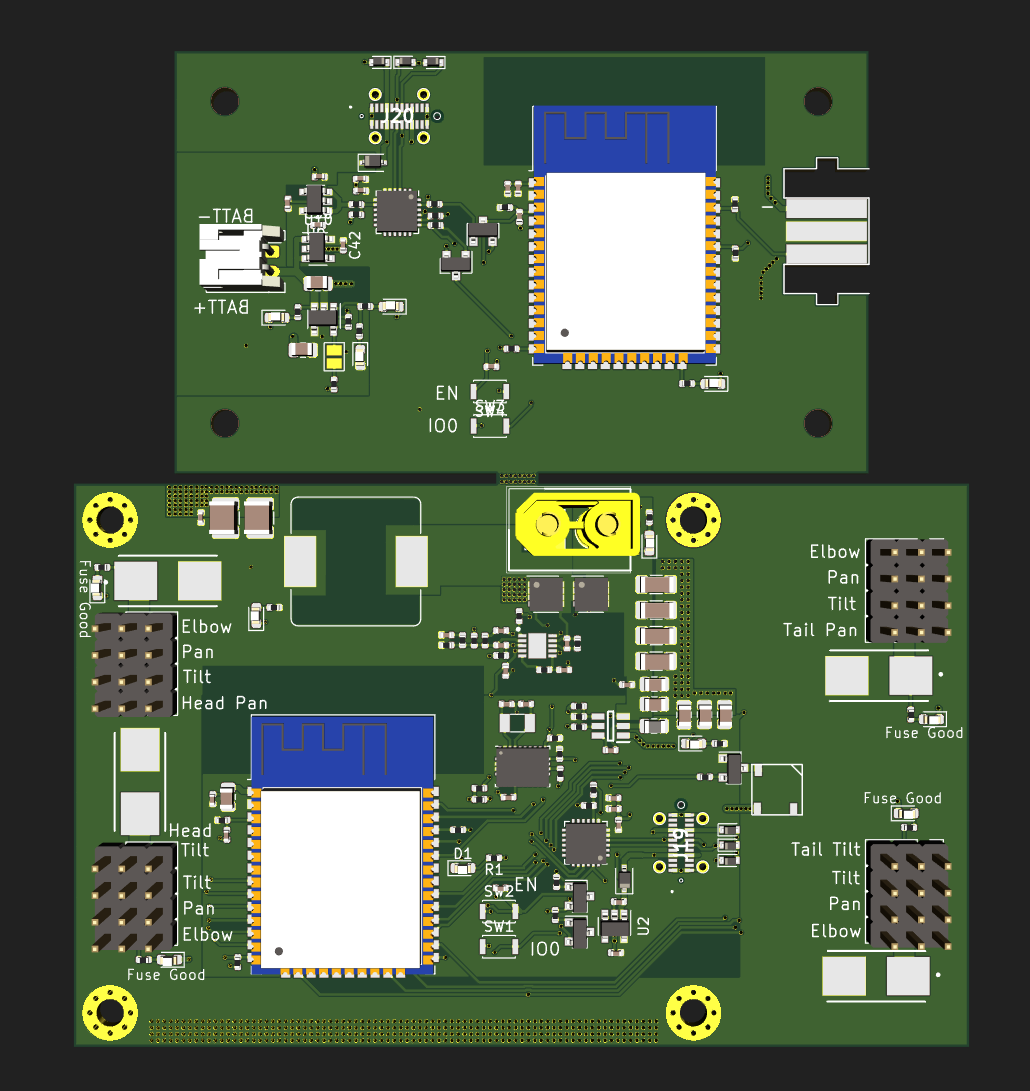
\includegraphics[width=0.4\textwidth, height = 0.28\textheight, keepaspectratio]{Images/Motherboard.png}};
% \draw [white, rounded corners=\ClipSep, line width=\ClipSep] 
%     (current bounding box.north west) -- 
%     (current bounding box.north east) --
%     (current bounding box.south east) --
%     (current bounding box.south west) -- cycle
%     ;
% \end{tikzpicture}
%   	\caption{Motherboard}
% 	\label{fig:Motherboard}
% \end{figure}
    
%%%%%%%%%%%%%%%%%%%%%%%%%%%%%%%%%%%%%%%%%%%%%%%%%%%%%%%%%%%%%%%%%%%%%%%%%%%%%%%%
\subsection{Electronics Validation}

\subsubsection*{Testing Fixture}
In order to endure reliability of the developed motherboard and controller board a series of exposed test points along the reverse of both boards were placed in order for the board to be placed on a test fixture to confirm all the major sections of the board are working. The test points test the USB programming circuit on both boards, the $i^2c$ lines, a micro controller working pin and 3.3v is tested for both the mother board and the controller board. In addition to these, on the motherboard the ere are probe points to inject battery voltage, inspect the out put voltage for the integrated switch mode regulators and the battery voltage sense circuit. in order to easily and quickly test these boards a mirrored board was developed using spring loaded pins with a micro controller and serial programmers onbaord. A fixture that this board is mounted into was then designed and 3D printed to allow for quick insertion and removal of the board under test. A series of leds was added to act as confirmation lights with different ones turning on or off for different things under test for each board. The testing procedure can be seen in appendix[\ref{appendix:TestingProcedure}]

\subsubsection*{Safety}
    In designing the system, great caution had to be taken with the lithium ion battery in the system. In order to keep the system safe, a series of fuses were integrated into the motherboard to prevent from short circuits or failures of motors. In addition to this current sensors have been added to each motor to determine major stall states to prevent complete failure of the motor. In addition to these a secondary micro controller was implemented as a safety system. This micro controller will monitor battery voltage, charge state, battery charging and battery balancing to ensure each cell is evenly charged to ensure longevity and safety. This micro controller will also  maintain control over the onboard power regulators and will be able to turn them on or off in a series of cases. This micro controller will remain on and in low power mode while the robot is turned off or the battery is too low to be used safely. In order to safely charge the battery pack, a charging system utilizing USB power delivery was implemented along with a cell balancing and monitoring system. 
%%%%%%%%%%%%%%%%%%%%%%%%%%%%%%%%%%%%%%%%%%%%%%%%%%%%%%%%%%%%%%%%%%%%%%%%%%%%%%%%
\subsection{Software Design Considerations}
\paragraph*{Mechanical}
    When designing the mechanical system for the robot, there were large number of constraints and hurdles to overcome. Many of the constraints can be refined down to the cost and the size constraints set forth during the development of the platform. 
    \begin{itemize}
        \item Motor selection- 
            When deciding motors to use there were a number of criteria to compare. 
            \begin{itemize}
                \item Size
                \item Torque
                \item Power requirements
                \item Availability
            \end{itemize}
            In end the 13g servo form factor was chosen for the size as it would allow the overall robot size to remain small and light as can be seen in [\ref{appendix:MotorSelection}]. It then came to choosing the specific motor to use, it came down to 4 motors. All of the considered motors were high torque variants using metal gears. due to sharing the same form factor they all remained in a very similar volumetric size so it came down to which motor would be most capable and reliable. After testing with all of the considered motors, the final motor chosen was the MG90B for its high size to torque ration, being far higher than the other options.\newline
        
        \item Manufacture-ability
        While designing this robot a great deal of time was spent in designing for manufacture-ability. Each method of manufacturing has different constraints in what can be produced successfully, efficiently and quickly. When designing a number of factors were considered. \newline
            \begin{itemize}
                \item Manufacturing style
                \item Number of components
                \item Production cost
            \end{itemize}
        The primary means of manufacturing was chosen as 3D printing because it would allow the robot to be iterated quickly and available to the most people. However for mass production of the platform, a series of molds would be created and parts would be cast using a poly-urethane resin. This required all parts to be designed with both in mind ensuring there were as few areas with unreachable overhangs, parts could be placed flat in order to reduce the amount of support material while printing and many other details. By choosing these two methods of manufacturing the overall production costs are kept very low.\newline
        Due to the nature of the system, there will be a high number of individual components (79 total parts in the final design), by reusing the same piece in multiple it both reduces the complexity of assembly and the total number of models that have to be manufactured. Through this technique, the robot was able to be designed out of 22 individually unique components which would be able to be printed in 3 cycles of a standard 200mm x 2000mm 3d printer (industry standard for non industrial printers).\newline
        \item Assemble-ability
        While manufacture-ability encapsulates the majority of the design process, the means of assembling was also considered carefully. The ability to put the robot together quickly and easily is critical. By analyzing the process taken to assemble an early prototype of the robot and adjusting the design the assembly time was reduced from \approximately 5hrs to \approximately1.5hrs. The final revision of the design utilized 2 lengths of m3 bolts and their corresponding nuts to assemble the whole robot. The use of 2 lengths of screws also drastically reduces the cost. 
        
    \end{itemize}
\paragraph*{Electrical}
The electrical system came down to a few major requirements. The robot requires many independent sub components with their supporting hardware

    \begin{itemize}
        \item Micro controller -
            When choosing the micro controller there were a few requirements set forth, it would have to be able to run 16 independent PWM channels through hardware, communicate through either USB-HID or UDP and have a dedicated hardware $i^2c$ bus. With these requirements a list of possible micro controllers was developed, ranging from off the shelf boards to completely custom hardware.
            \begin{enumerate}
                \item Teensy 3.5/3.6
                \item Teensy 4.0
                \item ESP32
                \item STM32
            \end{enumerate}
            From this list a custom motherboard was developed. From this list of micro controllers it was narrowed down to two choices being the Teensy 3.5 and the ESP32, one option providing hardware USB-HID and the other UDP. From this a final version of the motherboard was developed using the available boards. Both boards were then put into robots for testing. The ESP32 communicating directly with the high level controller over WiFi, the Teensy communicating with a Raspberry pi onboard the robot, running the high level controller. However due to a bug in the current Raspberry pi kernel and the USB HID library implemented in have the testing on the Teensy had to stop as it could not be tested in the assembled system in the intended way. This switch also reduced the overall price of the system by removing the cost of a dedicated Raspberry Pi and by using a much lower cost micro controller.\newline
            
        \item IMU- 
            The IMU chosen was the BNO055 as it contains an embedded M0 arm micro controller that filters the data coming out of the IMU. This allows the system to have a much more reliable source of data. The internal micro controller is also able to provide a gravity vector and the Euler angles within each axis of rotation.\newline
            
        \item Power regulation-
        Due to the power requirement of the motors chosen, a consistent 6v power supply with about 20A continuous current draw is required. 6v is a very uncommon voltage supply with 2s lithium batteries coming in at a nominal 7.4V and most bench power supplied only supplying up to 10A. In order to increase the battery life capacity without increasing the size of the cells as well as allowing for higher voltage power supplies with lower current ratings to be used a high current switch mode supply was designed with up to an 18V input and up to 20A output. With an overall efficiency of about 85\% at the full 20A draw the onbaord supply is highly efficient at converting high voltage, low current supplies down to 6v at the required 20A. \newline
    \end{itemize}
    During the development stages of the motherboard, off the shelf development boards and modules were used for the micro controller, IMU and power regulation. This drastically increased the overall cost of the electronics in the system. Once the system was proven and tested, the final revision of the motherboard was designed and resulted in a cost reduction of about 80\%. In addition to the cost reduction, The overall number of through hole components was drastically reduced, making it marginally easier to produce.
In choosing the language, development environment and in turn some of the electronics and hardware a number of things had to be considered. The primary list of languages for this High level control development include
\begin{itemize}
    \item C/C++
    \item Java
    \item Python
    \item Matlab
    \item GO
\end{itemize}

The Same design decisions that went into the High level development environment had to be considered for the micro controller level Embedded code, however there was a different set of available languages for the micro controller we choose. The well supported of which include:
    \begin{itemize}
        \item Micro Python
        \item C/C++
    \end{itemize}
\subsubsection*{High Level Control}
\paragraph*{Language Commonality}
In order to get a platform adopted the language used needs to be common and well supported, this therefor brings the list of languages down to Java, C/C++, Python and Matlab. These three languages encapsulate the top 48\% of most popular programming languages\cite{tiobe}. This leans they have a great deal of documented and community support and therefor can be debugged and developed easily.
\paragraph*{Operating System Support- High Level Control}
    While most languages are supported by Mac OS, Linux and Windows, some are far easier to compile and get working than others. In order to make the start up process as easy and seamless for the end user, a language that could be pre-compiled or did not require specialized packages to compile would be chosen. This reduced the language choice for the high level controller to either Java, Python or Matlab.
    
    Due to the requirement of a Matlab license to use the program to its full potential it was eliminated. 
\paragraph*{Development speed}
    With the nature of classes and labs, development time and learning curve is a key concern, students should be learning the concepts of the class and not a new language. In this Python is the clear leader, it has the lowest learning curve as well as the lowest development time. However Java has a number of scripting languages such as Groovy, Kotlin and PyJava. These drastically reduce the development time of java while still allowing the user to integrate pure java code with out issues at compilation and run time. Meaning both Java and Python are strong language contenders int his regard.

\paragraph*{Run time speed}
In order to get a reliable dynamical controller run at a high level it was important to have language that could have full system resources allocated to it. It was also important that the language was able to run in a real time-esq system where a set of code could be run on a high frequency interval with reliability and this could be done on any system without having an effect from other code. In this case Java was the final choice as the 'Niceness' of the program could be adjusted to prevent other system processes from affecting the run time of the program. This in combination with the object oriented nature of the language makes development and implementation of features very easy for the instructor and students.\newline


Due to all of these considerations Java was chosen as the primary language for back end development and for script and gait development a Java based scripting language called Groovy will be supported, however any java based scripting language will work and/or Java itself will work in the same manner. \newline

\subsubsection*{Micro-Controller}
\paragraph*{Micro Python}
    Micro Python is an implementation of python developed for micro controllers, running naively on board. Using micro python comes with all the benefits of python such as the ease and speed of develop-ability but also comes with many draw backs as it can be less efficient than some of its counterparts. Configuring the ESP32 to run Micro Python requires quite a bit of effort to be put forth to configure however once configured it will persist. The major draw backs of micro python are there are no dedicated development environments tailored to the language and the libraries for the micro controller platform. This means it becomes very difficult to support the platform and update libraries and requirements change over time.
\paragraph*{C/C++}
    In the Realm of C/C++ for the ESP32 there are two major options, using the Arduino ide and its integrated framework of using the ESP-idf (integrated development framework) provided by the manufacturers of the ESP32 Espressif. Each platform has its advantages and disadvantages. Arduino is very easy to install, comes with a number of supported libraries and can be easily distributed to and updated however comes with some performance disadvantages due to internal overheads of the framework itself. The ESP-idf is very difficult to install with inconsistent operating support, no centralized library and package manager and may be very daunting as it is a HAL(hardware abstraction library) meaning it is only one step above the pure embedded level of the code for the micro controller, however due to the idf being a HAL, it is very efficient as avoids many of the overhead problems encountered by Arduino.
    Both the ESP-idf and the Arduino ide have support for all the required features for this platform and many more. Importantly both integrate the RTOS(real time operating system) developed for the ESP32 to handle the WiFi and any system level interrupts making it much easier for the end user not to have to implement this themselves. \newline\newline
In End C/C++ through the Arduino ide was chosen due to the efficiency of the system, the integrated RTOS and availability of documentation and support and the overall efficiency of the language in comparison to Micro Python. The Arduino environment was chosen over the integrated development framework due to the ease of setup and deliver-ability of the code, libraries can be easily updated and the code can be easily refreshed with little to no user input for sample and starter code.


    This paper has introduces the SmallKat robotic quadruped platform, the capabilities of the platform and the design criteria utilized when creating the platform. The resulting platform was capable of performing a number of educational concepts including kinematics, trajectory planning, gait generation, controls and dynamics. This platform can allow for institutions and research labs to develop and teach with a capable platform. This will assist in the development of multi-pedal systems in the field of robotics as a whole by creating more engineers with experience in the field.
    The final platform is a combination of custom electronics and off the shelf servo motors. This combination allows for a reliable yet affordable platform. With the safety features integrated and the pedagogical objectives integrated into the design allow the system to be ideally suited for research and teaching within a lab setting. With most large quadruped platforms the robot has enough force to break itself or injure a user working on it, SmallKat has enough torque to walk but has safety features integrated and utilizes motors with low enough torque that it is unable to damage itself or the end user in any meaningful way.
\section{Results}
\label{sec:results}
A series of tests were run to compare the robots ability to perform tasks required for the teaching objectives listed in section \ref{sec:DesignReqs}. In order to prove the robots ability to correctly demonstrate forward and inverse kinematics and to ensure the kinematic equations being used were accurate, high accuracy magnetic encoders were attached to the joints and the joint angles recorded through out the actions. In order to prove the inverse kinematic of the system, an initial reachable point in a legs work space was given and a second point in the work space  and the path the leg followed is compared to the theoretical, straight line path between the two points is shown in figure \ref{fig:IK}

    \begin{figure}[H]
	\centering
      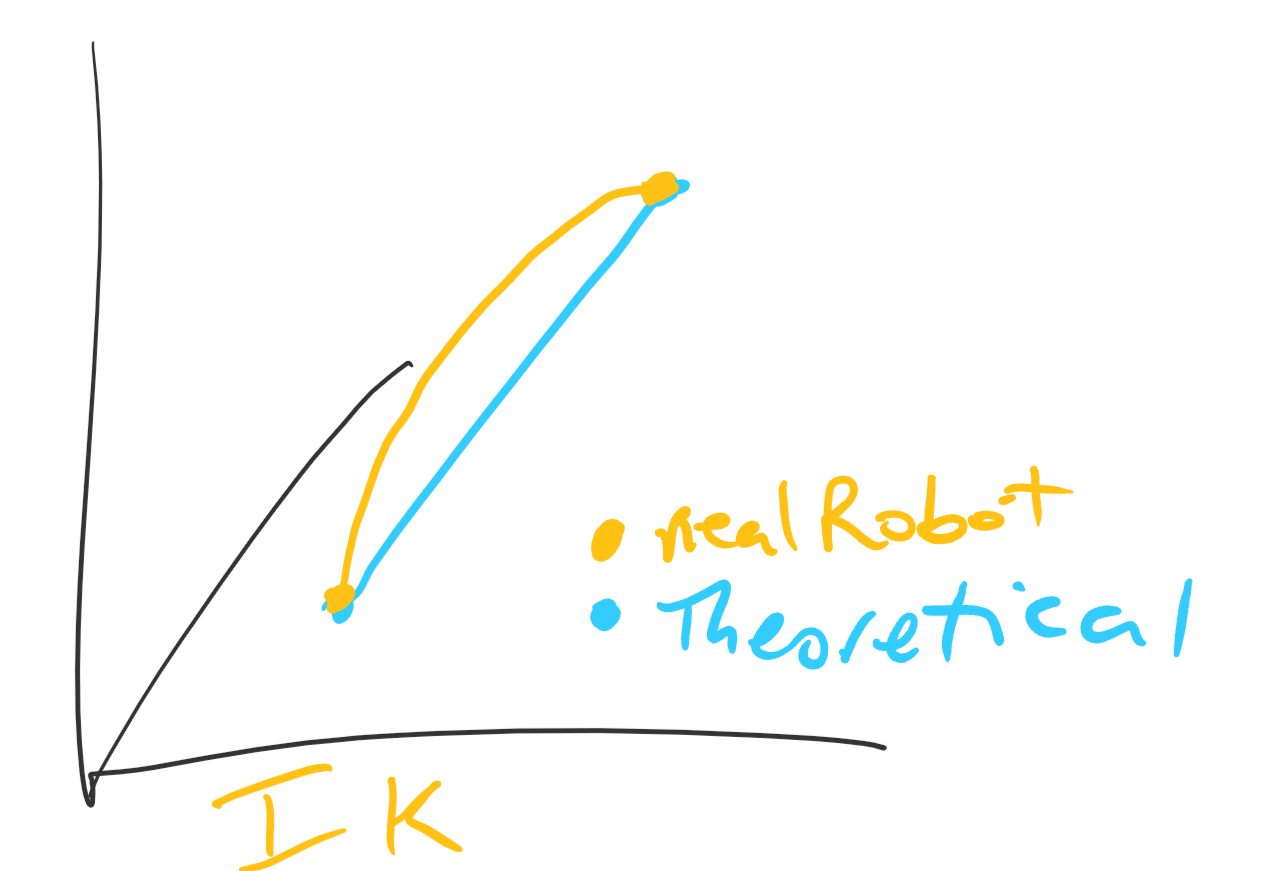
\includegraphics[width=0.4\textwidth]{Images/ik.png}
  	\caption{Graph showing the theoretical vs real trajectory in Inverse Kinematics}
  	\label{fig:IK}
\end{figure}

Using the same joint angles collected at the initial location and final location the forward kinematics were calculated to ensure the end effector was in the right location. To ensure correctness the forward kinematics were calculated using both the geometric approach and the DH approach. The calculations of which can be seen in equations \ref{eq:testfkgeometric} and equation \ref{eq:testfkDH} respectively.
\begin{eqfloat}[H]
$$
        \begin{aligned}
            3(a-x) = 3.5x + a - 1           \\
            3a - 3x = 3.5x + a -1           \\
            a = \frac{13}{4}x - \frac{1}{2} 
        \end{aligned}
$$
\caption{\label{eq:testfkgeometric}Forward kinematics Geometrically solved}
    
\end{eqfloat}

\begin{eqfloat}[H]
$$
        \begin{aligned}
            3(a-x) = 3.5x + a - 1           \\
            3a - 3x = 3.5x + a -1           \\
            a = \frac{13}{4}x - \frac{1}{2} 
        \end{aligned}
$$
\caption{\label{eq:testfkDH}Forward kinematics DH approach solved}
\end{eqfloat}

Following these tests, testing the ability to follow a given trajectory using a single leg. This was done by generating a trapezoidal trajectory path, similar to that used in the gait generation algorithm with way points along the path. These way points were then used to generate trajectories between the points. The trajectories were then broken into segments and passed in to the inverse kinematic equations and passed to the robot. In the same way the joint angles were collected for the inverse kinematics test, the encoders were used to collect the joint information. This comparison can be seen in figure \ref{fig:Trajectory}

    \begin{figure}[H]
	\centering
      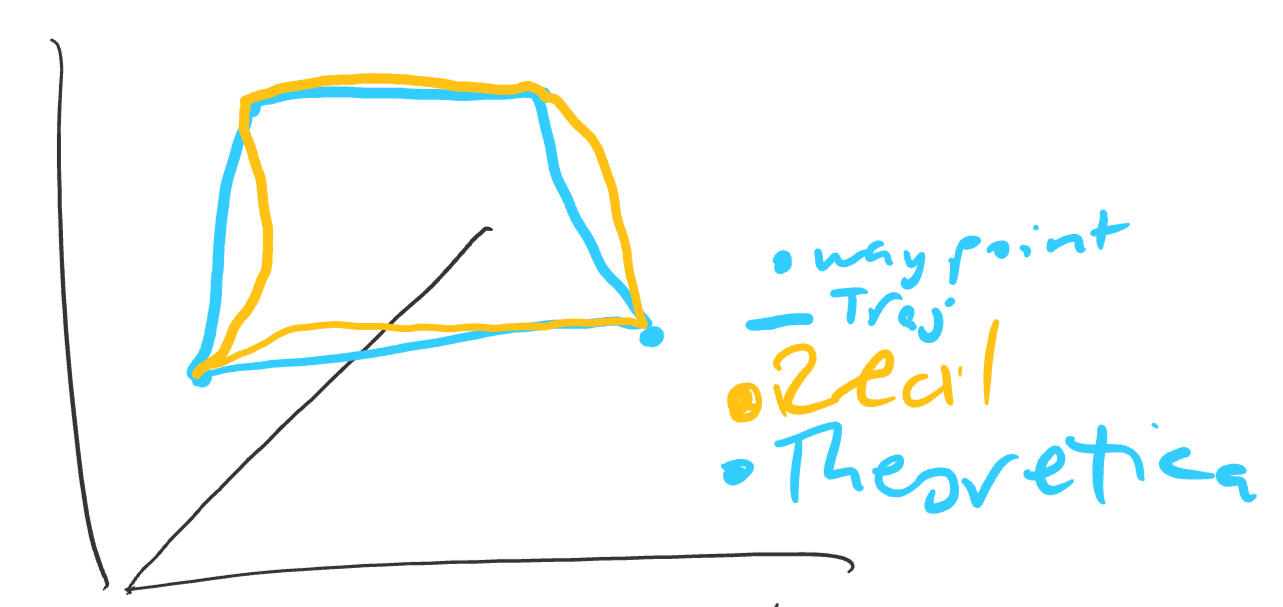
\includegraphics[width=0.4\textwidth]{Images/trajectory.PNG}
  	\caption{Graph showing the theoretical vs real trajectory}
  	\label{fig:Trajectory}
\end{figure}

To prove the robots ability to perform a generated gait was validated by pre computing a static walking gait and passing it to the robot and having it follow each generated trajectory of each leg. The results of this can be seen in figure \ref{fig:gait}
    \begin{figure}[H]
	\centering
      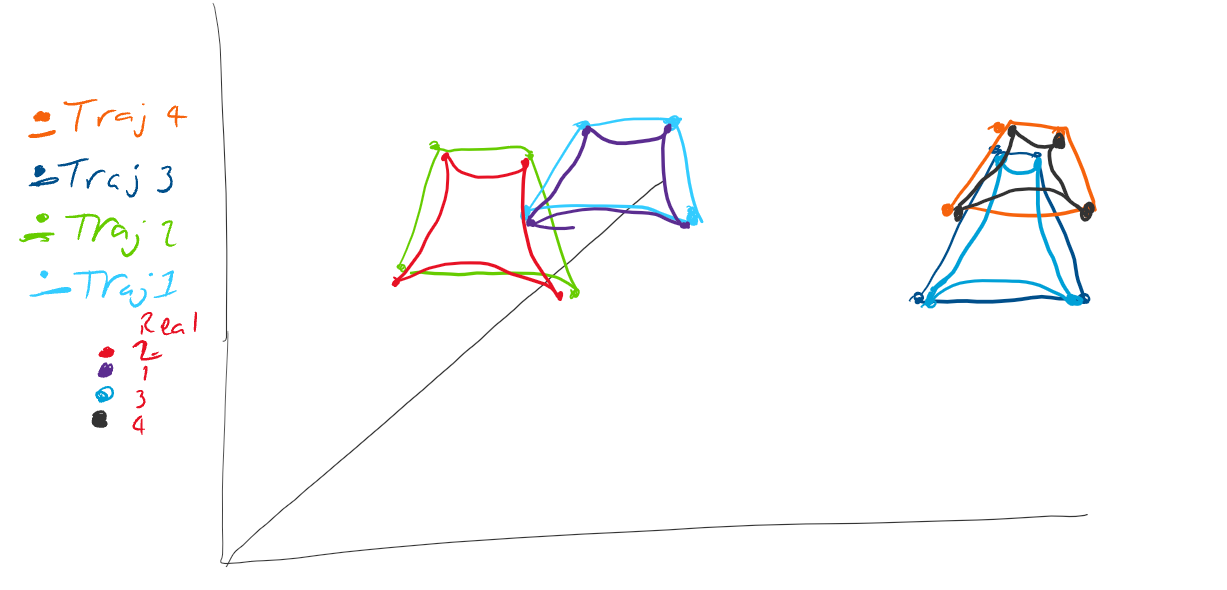
\includegraphics[width=0.4\textwidth]{Images/gaits.PNG}
  	\caption{Graph showing the generated gait vs real gait}
  	\label{fig:gait}
\end{figure}
\section{Conclusion}
As can be seen in the Section \ref{sec:resuls} the robot designed is able to successfully and accurately perform all tasks required in the defined teaching objectives in \ref{sec:DesignReqs}. The resulting robot and simulation developed are able to perform static and basic dynamic walking gaits with optimal operator safety. The over all robot was designed to meet a low cost price point in order to make it feasible as a lab kit for colleges and universities to further expand their course offerings. The targeted price point for the completed system including charging, battery and all related electronics similar to that of the turtle bot Burger being \approximately\$550. Both robots operate in a similar environment, both focusing on the educational and the research and development space.  



















                                  
\begin{appendices}
\section{Motor Selection}

\label{appendix:MotorSelection}

    \begin{enumerate}
        \item MG90D
        \item MG92B
        \item MG90S
        \item TGY-9018MG
    \end{enumerate}
    All of these motors were high torque variants using metal gears. due to sharing the same form factor they all remained in a very similar volumetric size so it came down to which motor would be most capable and reliable.
    \begin{figure}[H]
	   \centering
       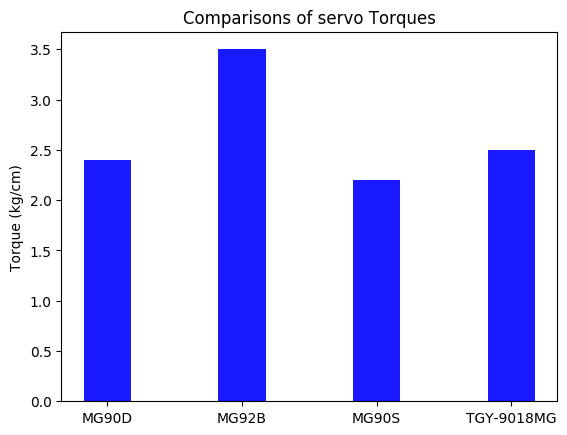
\includegraphics[width=0.4\textwidth]{Images/Motors.png}
  	   \caption{Torque values of different motors}
	   \label{fig:Motor_Torques}
    \end{figure}

\section{Testing Procedure}
\label{appendix:TestingProcedure}
\begin{enumerate}
    \item Plug in both USB cables for ESP32 programmers on jig
    \item Plug in communication USB for onboard micro controller
    \item Run Python test script
    \begin{enumerate}
        \item Program controller board with test firmware
        \begin{enumerate}
            \item Test for 3.3v regulation, $i^2c$ communication and micro controller status
            \item If passed program with final firmware
        \end{enumerate}
         \item Program Motherboard with test firmware
         \item Enable Battery power input
        \begin{enumerate}
            \item Test for 3.3v regulation, 6v regulation and battery monitoring circuit
            \item Test $i^2c$ communication to the micro controller
            \item Test $i^2c$ communication to the IMU
            \item Check micro controller status
            \item If passed program with final firmware
        \end{enumerate}
    \end{enumerate}
    \item Display a Pass/Fail status of the board, with reason of failure    
\end{enumerate}
\end{appendices}

\section*{Acknowledgment}

\bibliographystyle{IEEEtran}
\bibliography{bibliography}

\end{document}

